\section*{Methodology}
\label{sec:methods}

% If going for Nature Astronomy this will have descriptions on the code or so.
\paulo{Keep detailed calculations here.}

\paulo{We are allowed 10 extended figures, so we should use them if we can.}


\subsection*{Simulations}
\label{ssec:sims}

To establish the universality of our proposed Gompertz curve for the
neutral hydrogen reionization and discover its relationship with
cosmological parameter, we conducted 128 \texttt{21cmFASTv3}
simulations to generate the corresponding $x_\HI(z; \vtheta)$ profiles.
Our parameter space include $\vtheta = \{\sigma_8, \ns, h, \Omegab,
\Omegam, \zetaUV\}$, comprising five cosmological and one astrophysical
parameters.
The selection of $\sigma_8$ instead of $\As$ is imposed by the input
requirements of \texttt{21cmFAST}.
We use a scrambled Sobol sequence \cite{Sobol1967, Owen1998} to sample
quasi-uniformly in the $\vtheta$-space, with the following lower and
upper bounds:
%
\begin{alignat}{3}
\sigma_8 &\in (0.74, 0.90), &\quad
\ns &\in (0.92, 1.00), &\quad
h &\in (0.61, 0.73), \nonumber\\
\Omegab &\in (0.04, 0.06), &\quad
\Omegam &\in (0.24, 0.40), &\quad
\zetaUV &\in (15, 30).
\end{alignat}
%
The 1D and 2D projections of the distribution of our simulations is
displayed in \Cref{fig:sobol}.

The ionization efficiency $\zetaUV$ governs the ability of ultraviolet
photons to escape their parent galaxies and ionize the IGM.
Due to significant uncertainties surrounding $\zetaUV$, we opted to use
a constant value \YL{in each simulation}.
Note that this choice was made for simplicity, but a more realistic
assumption might be that $\zetaUV$ is a function of halo mass
\cite{Park2019} or redshift.
However, our findings suggest that $\zetaUV$ plays a minor role compared
to the cosmological parameters.
In fact, the best performing symbolic regression expressions do not use
$\zetaUV$.

\begin{figure}
\centering
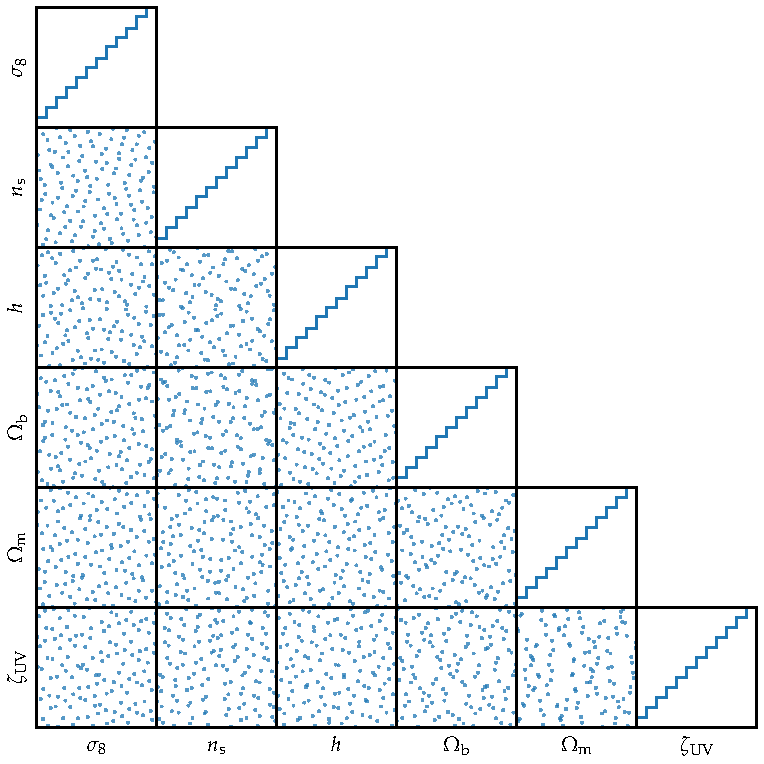
\includegraphics[width=25em]{figs/sobol128.pdf}
\caption{\textbf{Sobol sampling of our $x_\HI$ profiles}, in 6D
parameter space of $\sigma_8$, $\ns$, $h$, $\Omegab$, $\Omegam$, and
$\zetaUV$,
Each point in the lower triangular panels corresponds to the 2D
projection of a \texttt{21cmFAST} run, while the diagonal panels show
the 1D cumulative histograms for each parameter.
These 1D and 2D projections demonstrate the uniformity of our sampling
of the parameter space.}
\label{fig:sobol}
\end{figure}

Our \texttt{21cmFAST} simulations have a 300 comoving Mpc box size and
$768^3$ ($256^3$) cells for the matter (HI) field.
We maintain most options in their default values.

\paulo{We should probably mention the porosity vs mass-weighted concern
somewhere, also for methods perhaps?}


\subsection*{Inclusion of Helium reionization}
\label{ssec:helium}

The early intergalactic medium is primarily composed by neutral hydrogen
and helium.
Neutral helium (HeI) loses is first electron at the same time as neutral
hydrogen (HI) gets ionized \cite{Trac2007}.
However, there is a second reionization that occurs around $z\sim3$
where Helium (HeII) loses its remaining electron.

CMB photons will scatter off any free electrons, therefore both helium
reionizations contribute to the Thomson optical depth to reionization
$\tau_\reio$, although HeII ionization contribute relatively little in
comparison to HI and HeI ionizations \cite{Liu2016}.

To include the impact of the first helium reionization in our Gompertz
\texttt{CLASS}, we follow the approach used for the $\tanh$ model, i.e.\
the free electron fraction $x_\e$ is given by
%
\begin{equation}
\label{eq:xe_H_He}
x_\e = \Bigl(1 + \frac{Y_\He}{C (1 - Y_\He)} - x^\rec_\e\Bigr) x_\e^\Gomp + x^\rec_\e,
\end{equation}
%
where $Y_\He$ is the helium mass fraction, $C\approx4$ is the helium to
hydrogen mass ratio, $x_\e^\Gomp$ corresponds to the contribution of
free electrons due to \cref{eq:uni}, and $x^\rec_\e \approx
10^{-4}$ is the leftover free electrons from after recombination.

Given the relatively small impact on $\tau_\reio$, and the current
uncertainties regarding the timeline and the difficulty involved with
accurate modeling of HeII reionization \cite{Hotinli2023, Upton2020}, we
opted to follow the conventional approach and include HeII reionization
using the $\tanh$ model
%
\begin{equation}
\label{eq:xe_tot}
x_\e^\mathrm{Tot} = x_\e + \frac{Y_\He}{2C(1 - Y_\He)}
  \biggl(\tanh{\Bigl(\frac{z_\re^\HeII - z}{\Delta z^\HeII}\Bigr)} + 1\biggr),
\end{equation}
%
where $z_\re^\HeII = 3.5$ and $\Delta z^\HeII = 0.5$ are the midpoint
and duration of the second helium reionization, respectively.
These choices are also the default values used by \texttt{CLASS}.


\subsection*{Shape}
\label{ssec:shape}

\begin{figure}
\centering
\includegraphics[width=0.6\linewidth]{figs/shape_6.pdf}
\caption{\textbf{Universal shape of $x_\HI$.}
\emph{(Top)} 128 simulated $x_\HI$ timelines (thin light gray lines)
exhibit universality, after power-law transformations $\ar =
(a/\ap)^\tilt$.
The blue curves in all panels show our fitted analytic shape model, a
composition of the Gompertz curve with a 5th-degree polynomial in
\cref{eq:uni,eq:poly}.
\emph{(Middle)} Time derivative of $x_\HI$, can be interpreted as a PDF
if we view $x_\HI$ itself as the CDF.
We first discovered the universality by translating and rescaling each
$x_\HI$ using the mean and variance of its PDF, though now switch to the
better approach that jointly fits the global shape and individual
power-law parameters.
We use the latter as target of symbolic regression.
\emph{(Bottom)} Timelines transformed by the inverse of Gompertz
function, modeled in blue curve with a 5th-degree polynomial in
\cref{eq:poly}.}
\label{fig:shape}
\end{figure}

We find the shape with PySR by accide


\subsection*{\texttt{PySR} score}
\label{ssec:pysr}

SR learns from data using analytic expressions, unlike traditional
methods that adjust parameters in a fit.
Moreover, it can be employed to interpret deep neural network outputs
\cite{Cranmer2020b}.
\paulo{Yin, I added a simple SR intro, feel free to refine it here
before moving to the discuss the score.}

\paulo{Descibe here our choice for choosing between loss and
complexity.}


\begin{figure}
\centering
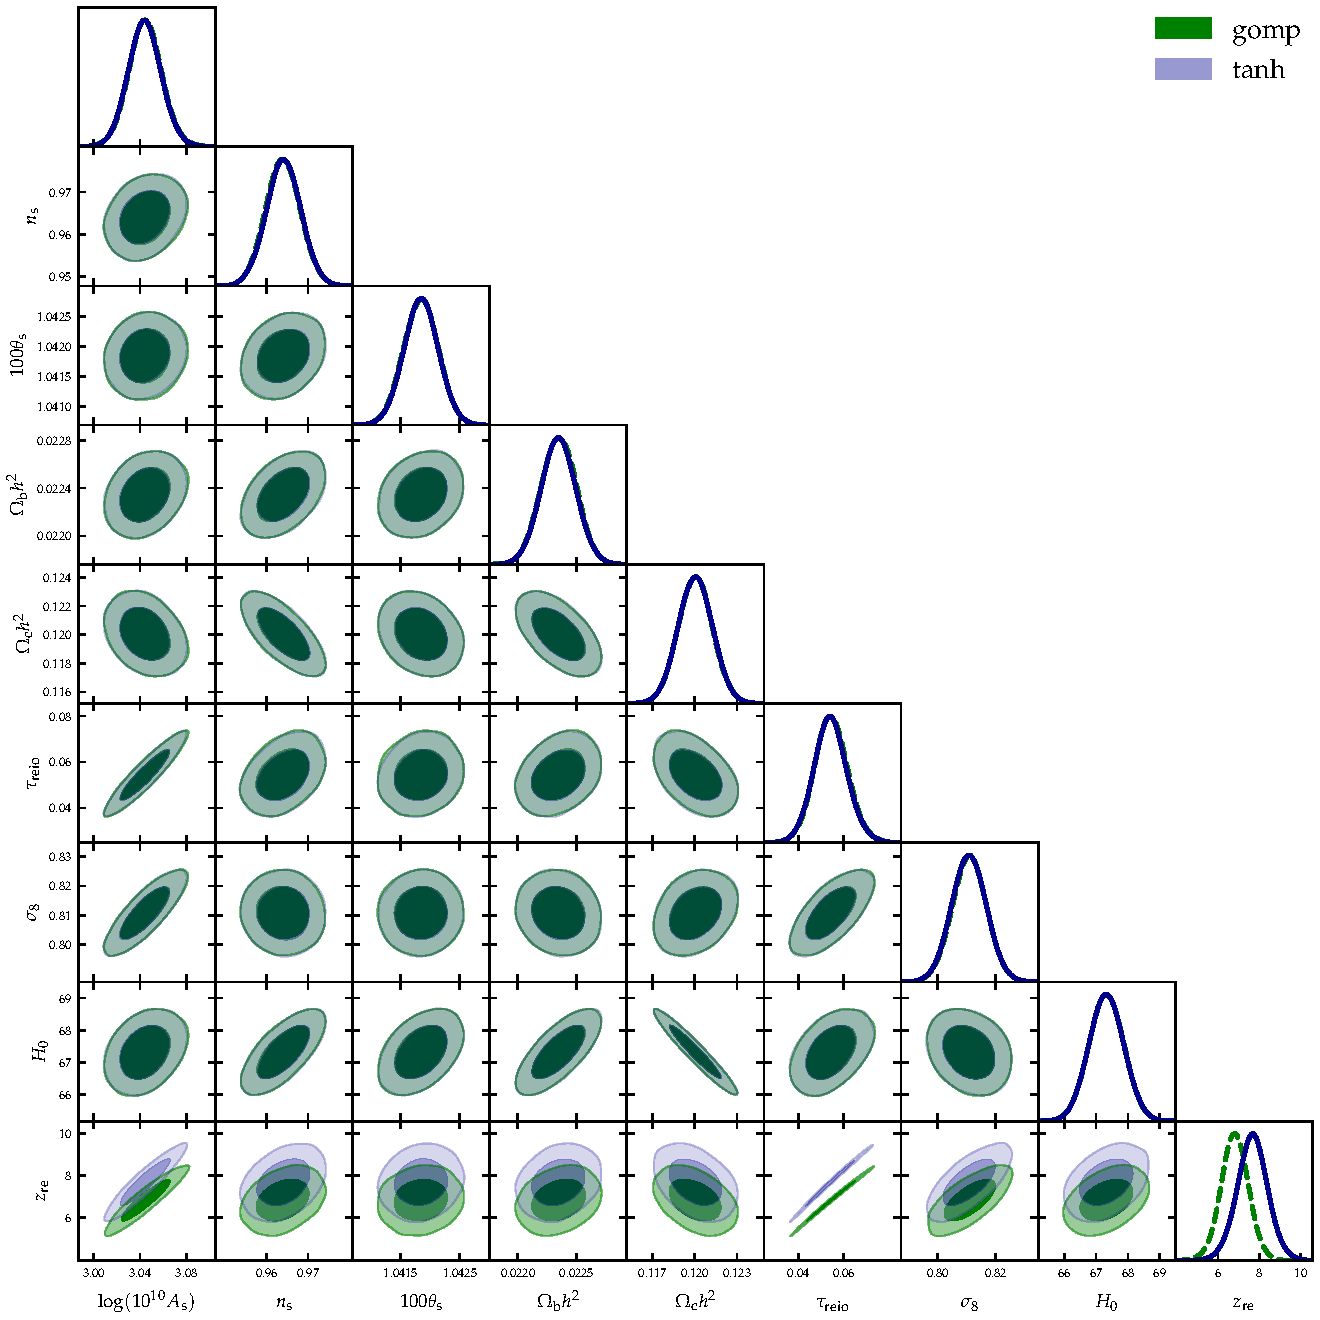
\includegraphics[width=\linewidth]{figs/gomp_tanh_triangle_tau.pdf}
\caption{\textbf{Analysis of CMB data with sampling over $\tau_\reio$
using both a universal shape for $x_\HI$ and the conventional $\tanh$
model.}
Note that we have not \emph{eliminated} $\tau_\reio$ from the analysis
yet.
Here, we use the standard choice of sampling over optical depth and
obtain the corresponding reionization history via bisection.
The green (blue) contours correspond to the constraints obtained with
our Gompertz universal shape ($\tanh$ model).}
\label{fig:tg}
\end{figure}

\begin{table}
\centering
\small
\begin{tabular}{llll}
\toprule
Parameter & Gompertz & $\tanh$ & Planck \\
\midrule
$10^{9} \As$ & 2.101 $\pm$ 0.031 & 2.099 $\pm$ 0.030 & 2.100 $\pm$ 0.030 \\
$\ns$ & 0.9638 $\pm$ 0.0041 & 0.9641 $\pm$ 0.0042 & 0.9649 $\pm$ 0.0042 \\
$\Omegac h^2$ & 0.1201 $\pm$ 0.0012 & 0.1201 $\pm$ 0.0012 & 0.1200 $\pm$ 0.0012 \\
$\Omegab h^2 $ & 0.02235 $\pm$ 0.00015 & 0.02235 $\pm$ 0.00015 & 0.02237 $\pm$ 0.00015 \\
$\Omegam$ & 0.3157 $\pm$ 0.0076 & 0.3157 $\pm$ 0.0076 & 0.3153 $\pm$ 0.0073 \\
$\Omegam h^2$ & 0.1430 $\pm$ 0.0011 & 0.1430 $\pm$ 0.0011 & 0.1430 $\pm$ 0.0011 \\
$\OmegaL$ & 0.6842 $\pm$ 0.0076 & 0.6842 $\pm$ 0.0076 & 0.6847 $\pm$ 0.0073 \\
Age [Gyr] & 13.800 $\pm$ 0.023 & 13.800 $\pm$ 0.023 & 13.797 $\pm$ 0.023 \\
$H_0$ & 67.32 $\pm$ 0.55 & 67.32 $\pm$ 0.55 & 67.36 $\pm$ 0.54 \\
$100 \theta_\mathrm{MC}$ & 1.04184 $\pm$ 0.00029 & 0.104815 $\pm$ 0.00029 & 1.04092 $\pm$ 0.00031 \\
$\sigma_8$ & 0.8109 $\pm$ 0.0059 & 0.8108 $\pm$ 0.0060 & 0.8111 $\pm$ 0.0060 \\
$S_8 \equiv \sigma_8 \sqrt{\frac{\Omegam}{0.3}}$ & 0.832 $\pm$ 0.013 & 0.832 $\pm$ 0.013 & 0.832 $\pm$ 0.013\\
$\tau_\reio$ & 0.0546 $\pm$ 0.0076 & 0.0543 $\pm$ 0.0075 & 0.0544 $\pm$ 0.0073 \\
$z_\re$ & 6.81 $\pm$ 0.68 & 7.67 $\pm$ 0.75 & 7.67 $\pm$ 0.73 \\
\bottomrule
\end{tabular}
\caption{\textbf{Parameter constraints from Planck CMB I.}
Summary table of the constraints and corresponding errors for
representative parameters of the universal shape (Gompertz) and $\tanh$
models.
The constraints use CMB `TTTEEE' + lensing information.
The results from the Planck analysis \cite{Planck2020a} are included for
comparison.
Note that we sample over $\tau_\reio$ and have not included the mapping
from cosmological dependence to reionization history in these results.}
\label{tab:tau_comp}
\end{table}


\begin{figure}
\centering
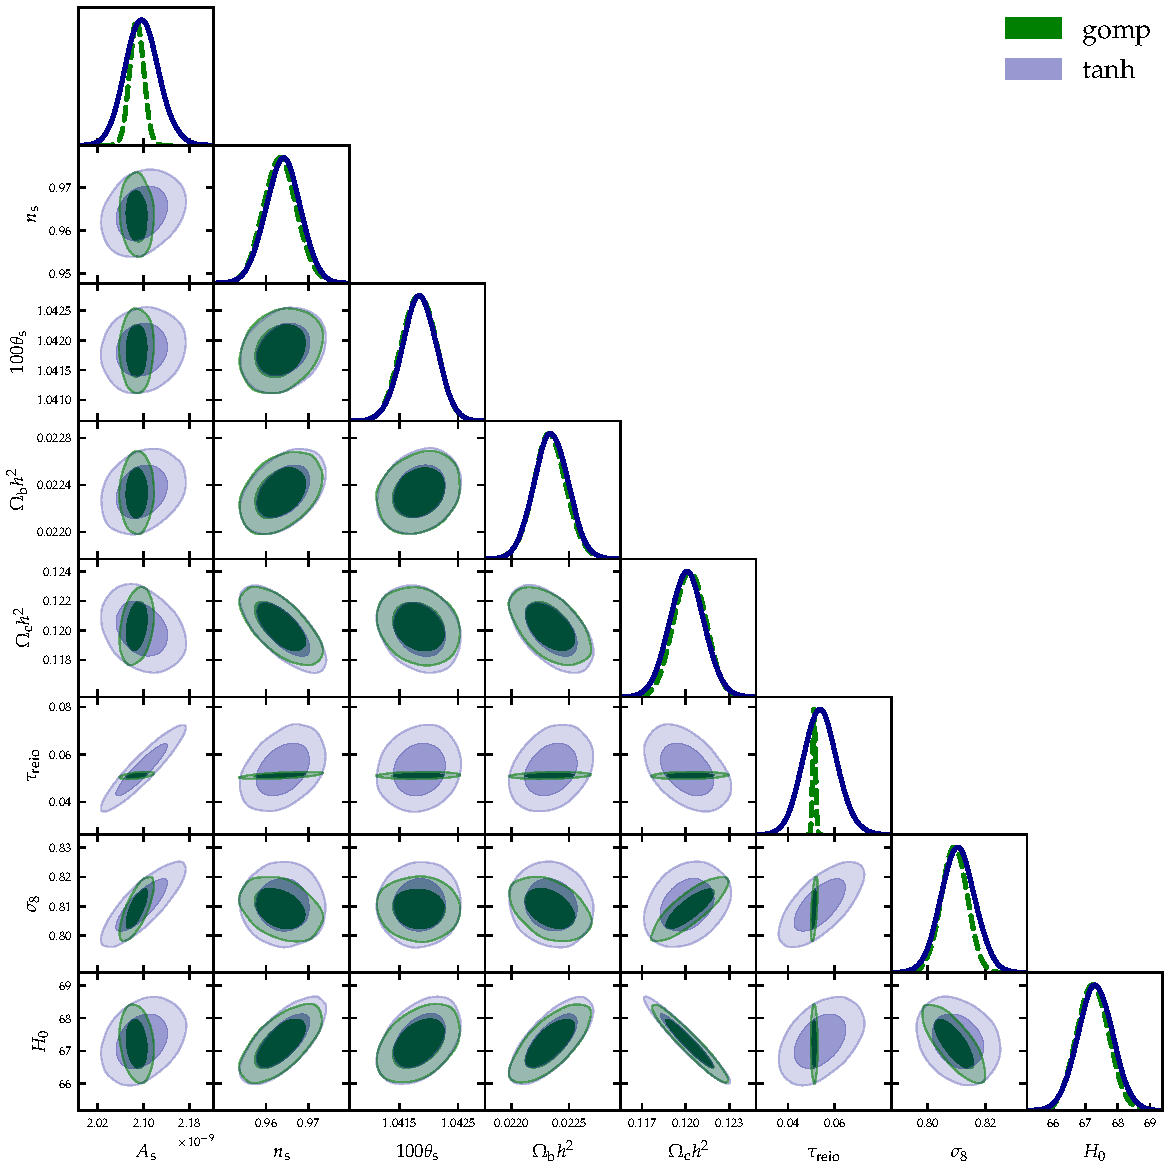
\includegraphics[width=\linewidth]{figs/gomp_tanh_triangle_kill_full.pdf}
\caption{\textbf{Analysis of CMB data with $\tau_\reio$ as a derived parameter using \cref{eq:SR} and the conventional $\tanh$ model (sampling over $z_{\rm re}$ for reference). } Here we combine our Gompertz universal shape with the rescaled pivot and tilt obtained via symbolic regression. Note that for the Gompertz model we do not sample over $z_{\rm re}$ since \cref{eq:uni} does not depend on it. The green (blue) contours correspond to the constraints obtained with
our Gompertz universal shape ($\tanh$ model).}
\label{fig:unleashed_gomp}
\end{figure}


\subsection*{\texttt{PySR} alternative mapping}
\label{ssec:0226}

The mapping between neutral hydrogen profiles and cosmology is not
unique.
Through a run of \texttt{PySR}, we generate families of expressions
capable of representing the simulated $x_\HI$ data with increasing
complexity and slightly improved performance (lower loss).
See \nameref{ssec:pysr} for details on selecting the best-performing
analytic expression.
Evidently, the resulting expressions for the tilt $\tilt(\vtheta)$ and
pivot $\ap(\vtheta)$ in \cref{eq:map}, obtained using symbolic
regression, depend on the available simulated data.

To investigate the impact of the sampling of simulated data, which
corresponds to the variance in the context of deep learning, we
construct an alternative mapping of reionization with cosmology using
only half of the \texttt{21cmFAST} $x_\HI$ profiles.
Once again, we find a constant tilt $\tilt = 8.331045$, remarkably close
to the value obtained using the full simulated data (8.289981).
This preference for constant tilt could be a consequence of the
astrophysical assumptions of reionization in \texttt{21cmFAST}.
A more complex simulation, such as one involving radiative transfer or
different X-ray preheating \cite{Montero2024}, might reveal a different
tilt.
Furthermore, the pivot is given by
%
\begin{equation}
\label{eq:SR0226}
\ln\ap(\vtheta) = (1.0389123 + \sigma_8) (\Omegab - \Omegam h  - \ns).
\end{equation}
%
Unsurprisingly, \cref{eq:SR0226} recovers the cosmological trends
present in \cref{eq:SR}.
Specifically, increasing $\ns$, $\Omegam$, and $\sigma_8$ leads to an
earlier reionization scenario, while a higher value of $\Omegab$
slightly delays reionization.
Furthermore, the impact of the Hubble constant is once again linked to
the matter density, albeit not in the same manner as in
\cref{eq:SR}.
This is likely evidence that the role of $h$ is limited, and
\texttt{PySR} considers its influence in conjunction with $\Omegam$
without increasing the complexity of the analytic expression.

\begin{table}
\centering
\small
\makebox[\textwidth][c]{\begin{tabular}{lllll}
\toprule
Parameter & Gompertz & Gompertz.5 & $\tanh$ & Planck \\
\midrule
$10^{9} \As$ & 2.088 $\pm$ 0.012 & 2.089 $\pm$ 0.013 & 2.098 $\pm$ 0.030 & 2.100 $\pm$ 0.030 \\
$\ns$ & 0.9634 $\pm$ 0.0040 & 0.9634 $\pm$ 0.0040 & 0.9641 $\pm$ 0.0041 & 0.9649 $\pm$ 0.0042 \\
$\Omegac h^2$ & 0.1203 $\pm$ 0.0011 & 0.1202 $\pm$ 0.0011 & 0.1201 $\pm$ 0.0012 & 0.1200 $\pm$ 0.0012 \\
$\Omegab h^2 $ & 0.02233 $\pm$ 0.00014 & 0.02233 $\pm$ 0.00014 & 0.02235 $\pm$ 0.00015 & 0.02237 $\pm$ 0.00015 \\
$\Omegam$ & 0.3171 $\pm$ 0.0068 & 0.3168 $\pm$ 0.0068 & 0.3159 $\pm$ 0.0075 & 0.3153 $\pm$ 0.0073 \\
$\Omegam h^2$ & 0.1433 $\pm$ 0.0010 & 0.1432 $\pm$ 0.0010 & 0.1431 $\pm$ 0.0011 & 0.1430 $\pm$ 0.0011 \\
$\OmegaL$ & 0.6828 $\pm$ 0.0068 & 0.6831 $\pm$ 0.0068 & 0.6840 $\pm$ 0.0075 & 0.6847 $\pm$ 0.0073 \\
Age [Gyr] & 13.803 $\pm$ 0.022 & 13.803 $\pm$ 0.022 & 13.800 $\pm$ 0.023 & 13.797 $\pm$ 0.023 \\
$H_0$ & 67.22 $\pm$ 0.49 & 67.24 $\pm$ 0.50 & 67.31 $\pm$ 0.54 & 67.36 $\pm$ 0.54 \\
$100 \theta_\mathrm{MC}$ & 1.04183 $\pm$ 0.00029 & 1.04183 $\pm$ 0.00029 & 1.04184 $\pm$ 0.00029 & 1.04092 $\pm$ 0.00031 \\
$\sigma_8$ & 0.8092 $\pm$ 0.0045 & 0.8092 $\pm$ 0.0046 & 0.8105 $\pm$ 0.0059 & 0.8111 $\pm$ 0.0060 \\
$S_8 \equiv \sigma_8 \sqrt{\frac{\Omegam}{0.3}}$ & 0.832 $\pm$ 0.013 & 0.832 $\pm$ 0.013 & 0.832 $\pm$ 0.013 & 0.832 $\pm$ 0.013\\
$\tau_\reio$ & 0.0511 $\pm$ 0.00061 & 0.0514 $\pm$ 0.00063 & 0.0538 $\pm$ 0.0074 & 0.0544 $\pm$ 0.0073 \\
$z_\re$ & 7.40 & 7.41 & 7.62 $\pm$ 0.74 & 7.67 $\pm$ 0.73 \\
\bottomrule
\end{tabular}}
\caption{\textbf{Parameter constraints from Planck CMB II.}
Similar to \Cref{tab:tau_comp} but including the cosmological mapping
to reionization histories.
Note that the midpoint of reionization $z_\re$ is not a derived
parameter of the model nor a sampled parameter in the Gompertz models;
instead, it is obtained directly with \cref{eq:uni}.
Furthermore, the $\tanh$ model included here samples over $z_\re$
instead of $\tau_\reio$.}
\label{tab:para}
\end{table}

Applying \cref{eq:SR0226} we reanalyze the CMB data following the
same approach as with \cref{eq:SR}.
The results are summarized in \Cref{tab:para}.
Comparing these findings to our previous results, we observe strikingly
similar values for all cosmological parameters, albeit with smaller
deviations from the Planck results.
The consistency between our results using the full $x_\HI$ data and
those using only half the data indicates that our symbolic
regression-based mapping performs well given the priors of our simulated
data (see \nameref{ssec:sims}).
